\documentclass{standalone}
% translate with >> pdflatex -shell-escape <file>

% This file is an extract of the PGFPLOTS manual, copyright by Christian Feuersaenger.
% 
% Feel free to use it as long as you cite the pgfplots manual properly.
%
% See
%   http://pgfplots.sourceforge.net/pgfplots.pdf
% for the complete manual.
%
% Any required input files (for <plot table> or <plot file> or the table package) can be downloaded
% at
% http://www.ctan.org/tex-archive/graphics/pgf/contrib/pgfplots/doc/latex/
% and
% http://www.ctan.org/tex-archive/graphics/pgf/contrib/pgfplots/doc/latex/plotdata/

\usepackage{pgfplots}
\usepackage{pgfplotstable}
\pgfplotsset{compat=newest}

% The manual loads these libraries globally; the extracted standalone examples
% need them too. external/clickable/snakes are intentionally omitted.
\usetikzlibrary{
	arrows.meta,backgrounds,calc,decorations.footprints,decorations.markings,
	decorations.pathreplacing,fixedpointarithmetic,intersections,patterns,
	plotmarks,shapes.arrows,spy,through}
\usepgfplotslibrary{
	colorbrewer,colormaps,dateplot,fillbetween,groupplots,patchplots,polar,
	smithchart,statistics,ternary,units}

% Some colormap examples reuse this display style defined earlier in the manual.
\pgfplotsset{
	cycle from colormap manual style/.style={
		x=3cm,y=10pt,ytick=\empty,
		colorbar style={x=,y=,ytick=\empty},
		point meta min=0,point meta max=1,
		stack plots=y,
		y dir=reverse,colorbar style={y dir=reverse},
		every axis plot/.style={line width=2pt},
		legend entries={0,...,20},
		legend pos=outer north east,
	},
}

\pagestyle{empty}
\usepackage{pgfplotstable}

\begin{document}
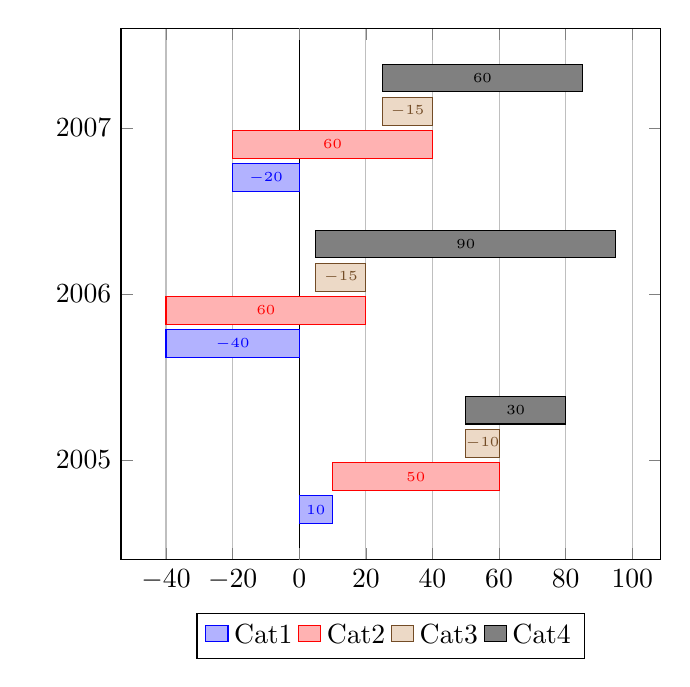
\begin{tikzpicture}
    \pgfplotstableread{
        Year  Cat1  Cat2  Cat3  Cat4
        2005  10    50    -10   30
        2006  -40   60    -15   90
        2007  -20   60    -15   60
    }\mytable
\begin{axis}[
    xbar stacked,
    stack negative=on previous,
    %
    xmajorgrids,
    legend style={at={(0.5,-0.1)},
        anchor=north,legend columns=-1},
    bar width=10pt,
    bar shift auto,
    nodes near coords,
    nodes near coords style={font=\tiny},
    y=60pt,
    ytick distance=1,
    enlarge y limits=0.3,
    /pgf/number format/1000 sep=,
    extra x ticks={0},
    extra x tick style={grid style={black},
    xticklabel=\empty},
]
    \addplot table [x index=1,y=Year] {\mytable};
    \addplot table [x index=2,y=Year] {\mytable};
    \addplot table [x index=3,y=Year] {\mytable};
    \addplot table [x index=4,y=Year] {\mytable};
    \legend{Cat1,Cat2,Cat3,Cat4}
\end{axis}
\end{tikzpicture}
\end{document}
